\chapter{Marco teórico}
\label{chap:teorico}
\cerradaarg{Falta mejorar ref y allref}
En este capítulo vamos a recorrer algunos términos básicos y problemas de procesamiento de lenguaje e information retrieval que deben conocerse para comprender mejor lo que discutiremos sobre question answering en los siguientes capítulos. En la primer sección vamos a introducir terminología básica como $token$, \textit{n-grama}, \textit{ontología} y $feature$, mientras que en la segunda veremos algunos problemas o áreas de procesamiento de lenguajes y recuperación de la información en los que los sistemas de question answering suelen apoyarse. Primero comentaremos qué es information retrieval, cuales son las métricas de evaluación del área y qué es un índice invertido de búsqueda, luego comentaremos los principales problemas propios de procesamiento de lenguajes relacionados con QA (POS tagging o etiquetado gramatical, NE tagging o reconocimiento de entidades y clasificación de preguntas) y finalmente, mencionamos algunas otras herramientas y conceptos de uso frecuente. 

\section{Terminologia}
\label{sec:terminologia}
\subsection*{Tokens}
\cerradaarg{Corta y endeble}
Un token es una palabra o un signo de puntuación en el contexto de un
texto.
Por ejemplo, el texto {\textquotedblleft}El sol
brilla.{\textquotedblright} tiene cuatro tokens:
\{{\textquoteleft}El{\textquoteright}, {\textquoteleft}sol{\textquoteright}, {\textquoteleft}brilla{\textquoteright}, {\textquoteleft}.{\textquoteright} \}. 
Las herramientas que generan una lista de tokens a partir de un texto se llaman
\textit{tokenizers} y suelen permitir distintos tratamiento de ciertas
palabras o signos de puntuación. (Por ejemplo: pasar todo a minúsculas, eliminar signos de puntuación, considerarlos aparte, etc).
Las bibliotecas que proveen tokenizers suelen proveer también herramientas para dividir un texto en
oraciones (\textit{Sentence Segmentation}). 
Estos dos procesos suelen ser el primer paso de todos los análisis de procesamiento de lenguaje natural.


\subsection*{N-Gramas}
\cerradaarg{Corta y endeble}
Un n-grama es una subsecuencia continua de \textit{n} tokens de un string.

Por ejemplo, la oración: {\textquotedblleft}Hoy está nublado{\textquotedblright}, tiene los siguientes n-gramas:
\medskip

\begin{tabular}{lll}
Tres unigramas & : & \{ {\textquotedblleft}Hoy{\textquotedblright}, {\textquotedblleft}está{\textquotedblright}, {\textquotedblleft}nublado{\textquotedblright} \} \\
Dos bigramas & : & \{ {\textquotedblleft}Hoy está{\textquotedblright}, {\textquotedblleft}está nublado{\textquotedblright} \} \\
Un sólo trigrama & : & \{ {\textquotedblleft}Hoy está nublado{\textquotedblright} \}\\
\end{tabular}
\medskip

Los n-gramas son útiles para recorrer un
texto con distintos tama\~nos de ventana en busca de algún patrón
conocido, por ejemplo: buscando entidades nombradas que no fueron reconocidas por otras herramientas.

{\color{red} Bajar a tierra on Google N-grams y POS de HMM}

\subsection*{Ontología}
\horrible
El término `ontología' es un término originalmente filosófico, que refiere al estudio de lo que hay, de lo que es, o, dicho de otro modo, a la definición y al estudio de los entes que existen en la realidad última y de sus cualidades esenciales y sus relaciones intrinsecas. Aplicado a ciencias informáticas, principalmente dentro áreas como inteligencia artificial y representación del conocimiento, esta noción original se sostiene, acotando la noción de realidad última a uno o varios dominios de problemas. Más concretamente, la noción de ontología en informática refiere a la definición formal y exhaustiva de un conjunto de conceptos que representan entidades, tipos o clases de entidades, propiedades y relaciones entre estas entidades relevantes para el modelado de un dominio de problemas dado. Esta ontología formal define un vocabulario inicial fijo que determina el tipo de problemas que se pueden plantear (y resolver) para el dominio.

{\color{red} Mencionar linked data, RDF, SPARQL, YAGO, dbPedia y Freebase. Está referido, revisar si lo borro.}

\subsection*{Features}
\label{subsec:features}
\cerradaarg{Sí, creo que sí}
En machine learning, un feature puede definirse como una propiedad medible de un fenómeno siendo observado. En las aplicaciones de procesamiento de lenguaje natural, el dominio de “fenómenos observados” está restringido a los fenómenos lingüísticos y las propiedades medibles también. Un ejemplo de feature es: un booleano indicando \dq{la palabra comienza con mayúscula}. En general, los features toman valores numéricos o booleanos, aunque también es posible utilizar features más complejos (como strings, o listas). Los features se agrupan en vectores. Durante un proceso de análisis, cada entidad procesada tiene un vector de features que la representa de manera tratable. Por ejemplo, podemos asignarle a cada palabra de una oración el siguiente vector de tres features:

\begin{center}
\begin{tabular}{ll}
$v_1$:$bool$ & indica si la palabra comienza con mayúscula \\
$v_2$:$int$ & indicando la longitud de la palabra \\
$v_3$:$string$ & representa la palabra en minúsculas \\
\end{tabular}
\end{center}


Encontrar features (o “características”) discriminantes e independientes entre si es una forma con la que se modelan correctamente muchos problemas de nlp, como la asignación de diferentes etiquetas a las palabras de una oración (por ejemplo: pos tags, ner tags), la clasificación de preguntas y la extración de tópicos. 

Los features aparecen en muchos contextos, por ejemplo: en \allref{chap:implementacion} nosotros construimos una serie de features a mano en la sección de answer retrieval, para subir la posición de la respuesta esperada entre la lista de pasajes rankeados. En las herramientas lingüísticas que veremos a continuación (\allref{sec:herramientas}), los features son normalmente extraídos automáticamente de un corpus. En estos casos, el volumen de features suele ser relativamente alto (10.000, 100.000) y se incorporan patrones estadísticos complejos alejados de la simplicidad del vector de tres features de nuestro ejemplo. 

A modo de ilustración, reproducimos los ejemplos que se pueden encontrar en \\ \cite{NER1} sobre dimensiones de features típicas para el proceso de reconocimiento de entidades. Veremos sobre reconocimiento de entidades en breve (\ref{subsec:nerc}), pero, brevemente, lo que se busca es encontrar entidades nombradas como \dq{Buenos Aires} o \dq{Juán Perez} en oraciones. En este proceso podrían usarse, por ejemplo, tres tipos de features basados en propiedades de las palabras mismas, en diccionarios conocidos y en propiedadades de los documentos del corpus.

\begin{center}

\begin{tabular}{|p {4cm} |p {10cm} |}
\hline
\multicolumn{2}{|c|}{Features a nivel palabra} \\ \hline
Features & Ejemplo \\ \hline
\multirow{3}{*}{Case} & Empieza con mayúscula \\
 &  La palabra está en mayúsculas \\
 &  Mezcla mayúsculas y minúsculas (por ejemplo: eBay, laTex) \\ \hline
\multirow{3}{*}{Puntuación} & Termina con punto, tiene un punto en el medio \\
& (por ejemplo: Sr., I.B.M.) \\
 &  Contiene un apóstrofre  \\ \hline
\multirow{2}{*}{Morfología} & Prefijo, sufijo, stem \\
 & Terminaciones comunes \\ \hline
Part-of-speech & nombre propio, sustantivo, verbo, etc \\ \hline
\multirow{5}{*}{Funcional} & Sólo letras, sólo símbolos, n-gramas \\
& Versión en mayúsculas / minúsculas \\
& Patrones (matchs con expresiones regulares) \\
& Cantidad de tokens, cantidad de carácteres \\ 
& Terminaciones comunes \\ \hline 
\end{tabular}

\begin{tabular}{|p {4cm} |p {10cm} |}
\hline
\multicolumn{2}{|c|}{Features sobre listas conocidas} \\ \hline 
Features & Ejemplo \\ \hline
\multirow{4}{*}{Lista General} & Diccionario general \\
 &  Stop words \\
 &  Sustantivos capitalizados (por ejemplo: Octubre, Lunes) \\
 &  Abreviaciones comunes (por ejemplo: Sr., PhD.) \\ \hline
 \multirow{3}{*}{Lista de Entidades} & Organizaciones, gobiernos, aerolineas, etc \\
 &  Nombre típico, apellido, celebridad \\
 &  Estrella, continente, país, calle \\ \hline
\multirow{3}{*}{Lista de pistas} & Palabras típicas de una organización ("asociados") \\
 &  Títulos, prefijos de nombres \\
 &  Palabras típicas de lugares ("río", "puerto") \\ \hline
\end{tabular}

\medskip

\begin{tabular}{|p {4cm} |p {10cm} |}
\hline
\multicolumn{2}{|c|}{Features extraídos de documentos} \\ \hline 
Features & Ejemplo \\ \hline
\multirow{3}{*}{Ocurrencias múltiples} & Entidades en el contexto \\
 &  Ocurrencias en mayúsculas o minúsculas \\
 &  Anáforas, correferencia \\ \hline
 Posición en documento & Posición según oración, parrafo, documento \\ \hline
\multirow{3}{*}{Metadatos} & URI, mail headers, sección del xml \\
 &  imágenes asociadas \\
 \multirow{3}{*}{Frecuencia en corpus} & Frecuencia de la palabra o la frase \\
 &  Co-ocurrencia \\
 &  Permanecia de una unidad de varias palabras \\ \hline
\end{tabular}
\end{center}


\section{Information Retrieval}
\label{sec:information-retrieval}
\label{subsec:information-retrieval}
\cerradaarg{Sin revisar igual}
El problema conocido como recuperación de la información (o \textit{information retrieval}) consiste, formalmente, en retornar \textit{información relevante} para una \textit{consulta} (\textit{information need}) a partir de una \textit{base de conocimiento}. 

Como la generalidad de esta definición sugiere, information retrieval es un área de trabajo amplia que abarca disciplinas variadas y problemas diversos (como por ejemplo: el almacenamiento físico de la información y su calidad, la representación de la información en modelos formales, el modelado semántico de las nociones de ``similaridad`` y ``relevancia`` entre las consultas de usuarios y los diferentes documentos de la base de información). 

El caso de uso socialmente más relevante y conocido son los motores de búsqueda web: en los motores de búsqueda, la base de conocimiento son las páginas de la web, la consulta es la cadeba de texto que ingresamos en el input del buscador, y la información relevante es una lista de documentos priorizados que, se espera, satisfará la necesidad de información del usuario. En estos sistemas, las consultas se interpretan como una serie de tokens concatenados con distintos operadores lógicos binarios, donde la barra espaciadora funciona como or inclusivo. El core del sistema es un \textit{índice de búsqueda} de los documentos de la base de conocimiento, que en principio podemos pensar como un diccionario indexado de palabras en documentos (más adelante veremos índices invertidos). El proceso de creación y mantenimiento de estos índices depende del tipo y del dinamismo de la base de conocimiento, y oscila entre un modesto setup a mano de una lista de documentos estáticos hasta el ejército de \textit{spiders} de google indexando la web en tiempo real. 

La consulta no es la necesidad de información del usuario sino lo que el usuario puede expresar de su necesidad dentro de la interfaz de consultas que el sistema de information retrieval sabe interpretar. Question Answering puede pensarse como un sistema de recuperación de la información que busca presentar una interfaz de consultas más cercana a la representación lingüística usual de una pregunta concreta y que entiende como información relevante una respuesta concreta en lugar de una lista de documentos. 

\subsection{Métricas}
\label{subsec:metricas-ir}
\cerrada{Sin revisar}
Las métricas de rendimiento de los sistemas de information retrieval articulan de diferentes maneras los documentos totales devueltos por el sistema, la cantidad de documentos relevantes y la cantidad de documentos irrelevantes para una consulta dada. En la práctica existen diferentes maneras de adjudicar relevancia a un documento. 

\begin{equation}\label{eq:precision}
 \mbox{Precisión}=\frac{|\{\mbox{documentos relevantes}\}\cap\{\mbox{documentos recuperados}\}|}{|\{\mbox{documentos recuperados}\}|} 
\end{equation}

\begin{equation}\label{eq:recall}
  \mbox{Recall}=\frac{|\{\mbox{documentos relevantes}\}\cap\{\mbox{documentos recuperados}\}|}{|\{\mbox{documentos relevantes}\}|} 
\end{equation}

\medskip 

Las dos métricas principales son la precisión y el recall.
La precisión \eqref{eq:precision} mide cuantos de los documentos devueltos son relevantes, la proporción de documentos relevantes en el total de documentos devueltos para la consulta. La precisión puede evaluarse sobre el total de documentos devueltos o sobre un corte arbitrario, considerando solamente los primeros $n$  resultados obtenidos. Por su parte, el recall\eqref{eq:recall} (traducido como \textit{exhaustividad}), mide cuantos de los documentos relevantes disponibles en la base de conocimiento fueron efectivamente recuperados. En general la precisión es la métrica privilegiada en casos de uso de sistemas de information retrieval. En QA, como veremos, las condiciones son diferentes.



Otras métricas conocidas son la familia de métricas $F$, que representa distintos trade off entre precisión y recall.
La formula general \eqref{eq:fb} introduce el parámetro $\beta$ que podera recall sobre precisión. $F_\beta$ pondera $\beta$ veces más el recall que la precisión. Las más utilizadas son $F_1$ (o solo $F$), $F_2$ y $F_{0.5}$. $F_2$ \eqref{eq:f2} pondera 2 veces más el recall que la precisión, por lo que es muy utilizada para evaluar subtareas de information retrieval en question answering.

\begin{equation}\label{eq:fb}
  F_\beta = \frac{(1 + \beta^2) \cdot (\mathrm{Precision} \cdot \mathrm{Recall})}{(\beta^2 \cdot \mathrm{Precision} + \mathrm{Recall})}
\end{equation}


\begin{equation}\label{eq:f2}
%  F = \frac{2 \cdot \mathrm{Precision} \cdot \mathrm{Recobrado}}{(\mathrm{Precision} + \mathrm{Recobrado})}
  F_2 = \frac{5 \cdot (\mathrm{Precision} \cdot \mathrm{Recall})}{(4 \cdot \mathrm{Precision} + \mathrm{Recall})}
\end{equation}


\subsection{Indice invertido de búsqueda}
\label{subsec:indice-invertido}
\faltapoco
Un índice invertido es la estructura de datos típica utilizada en problemas de information retrieval. Consiste en un mapeo de términos en documentos que los contienen. Es decir, para un término dado, un índice invertido devuelve una lista de los documentos cargados que lo contienen. Este tipo de estructuras invierte la relación normal en la cual a partir de un documento se accede a la lista de términos que este documento contiene (de allí el nombre invertido).
Por ejemplo, para los textos:
\medskip

\begin{tabular}{lll}
T[0] & = & ``qué es esto" \\
T[1] & = & ``esto es un ejemplo" \\
T[2] & = & ``qué gran ejemplo" \\
\end{tabular}
\medskip

Un índice invertido contendría las siguientes entradas (dónde el número \textit{n} es un puntero al texto T[n]):
\medskip %this skips a bit of vertical space

\begin{tabular}{lll}
	``qué" & : & \{0, 2\}\\
	``es" &:& \{0, 1\}\\
	``esto" & :& \{0, 1\} \\
	``un" & :&   \{1\} \\
	``ejemplo" & :& \{1, 2\} \\
	``gran" & :& \{2\} \\
\end{tabular}
\medskip
{\color{red} Mencionar un ejemplo de IR completo}

{\color{red} Mencionar otras estructuras de IR y quizas índices basados en LSA (link a LASSO?)}



\section{Procesamiento de Lenguaje Natural}
\label{sec:nlp}
\cerradaarg{No seamos perfeccionistas}

El problema de question answering puede pensarse como un problema de information
retrieval, pero en realidad excede este dominio: su objetivo no es devolver una lista de documentos para
una serie de palabras, sino una respuesta puntual a una pregunta
puntual. Para esto incorpora una dimensión semántica, esto es, toda
una serie de problemas de procesamiento de lenguaje natural que se
abordan con varias herramientas, que aportan distintos modelos de
análisis lingüístico a nivel \textit{oración}, tanto de la
consulta del usuario, como de los documentos indexados. Por ejemplo: el
pos-tagger es un analizador que genera la estructura gramatical de la
oración, mientras que \ el reconocimiento de entidades nombradas
(NER) identifica entidades como {\textquotedblleft}Buenos
Aires{\textquotedblright}, {\textquotedblleft}José
Pérez{\textquotedblright}, etc- y las clasifica (como \textit{lugar}
y \textit{persona}, respectivamente) . Los sistemas de QA utilizan
distintas herramientas para modelar la consulta y para buscarla, con
algún grado de comprensión semántica, dentro de su base de
conocimiento.
En lo que sigue de esta sección comentaremos algunas herramientas de procesamiento de lenguajes relevantes para question answering en general, y para nuestra tesis en particular.

\subsection{Part-of-speech (POS) tagging}
\label{subsec:pos}
\cerradaarg{No seamos perfeccionistas}
El POS-tagging o \textit{etiquetado gramatical} consiste en asignar a los diferentes 
tokens una etiqueta con el rol o categoría gramatical que cumplen en su contexto de emisión (por lo general, una oración o un párrafo). 
El POS-tagging cumple un rol fundamental en áreas como el reconocimiento de voz, el procesamiento de lenguaje natural e information retrieval.
El input de un pos tagger es una lista de tokens y un tagset (conjunto de etiquetas) específico, mientras que su output es un tag para cada uno 
de los tokens. Como ejemplo introductorio, consideremos la siguiente oración y un etiquetado gramatical posible:

\begin{center}
{\textquotedblleft}El hombre bajó la escalera.{\textquotedblright} 
\end{center}
\medskip

El resultado de un POS-tagger podría ser el siguiente:%\newline

\begin{center}
\begin{tabular}{| l | l |}
 \hline
Token & Etiqueta Gramatical (POS-tag) \\ \hline
El  & Determinante, artículo definido, masculino, singular\\ \hline
hombre &  Nombre común masculino singular (sustantivo) \\ \hline
bajó  & Verbo principal indicativo pasado tercera persona del singular (genero indefinido)\\ \hline
la  & Determinante, artículo femenino singular \\ \hline
escalera & Nombre común femenino singular (sustantivo) \\ \hline
.  & Punto final\\ \hline
\end{tabular}
\end{center}

La asignación de etiquetas no es un proceso trivial debido a la ambigüedad de roles posibles que tienen muchas palabras. Por ejemplo, la palabra
\sq{ayuda} puede funcionar como sustantivo (en \dq{La ayuda llegó a tiempo}) o como verbo (en \dq{Batman ayuda a los ciudadanos de Ciudad Gótica}). 
Un algoritmo de pos-tagging debe resolver estas ambigüedades seleccionando la categoría adecuada según el contexto. Más allá de estos casos, muchas palabras tienen una sola categoría posible (por ejemplo: \sq{ventana} es siempre un sustantivo, mientras que \sq{lentamente} es un adverbio y \sq{corrió} un verbo, etc).

Existen diferentes formas de clasificar gramaticalmente a las palabras. El esquema más general y reconocido de categorias gramaticales tal vez sea el siguiente, de 9 clases:
\begin{center}
\begin{tabular}{| l | l |}
 \hline
Categoría General & Ejemplos \\ \hline 
Determinante & aquel, este, mi, sus, nuestras \\ \hline
Pronombre & yo, tú, él, mí, nos, aquéllos, suyos \\ \hline
Preposición & a, ante, bajo, con, contra\\ \hline
Conjunción & y, aunque, pero, incluso\\ \hline
Interjección & ah, eh, ejem\\ \hline
Sustantivo & chicos, tesis, Pedro, cortapapeles\\ \hline
Verbo & cantamos, corrió, bailarán\\ \hline
Adjetivo & alegre, bonita, pésimos, desnuda\\ \hline
Adverbio & despacio, hábilmente, posteriormente\\ \hline
\end{tabular}
\end{center}

Mientas a algunas de estas categorías se les puede agregar más información, como \textit{género} y \textit{número} a los sustantivos, otras son categorías que no toleran modificaciones. Veremos esto con más detalle al hablar del tagset propuesto por el grupo EAGLES en breve.

Si bien en ciertos idiomas estas categorías no resultan del todo adecuadas o explicativas, dentro del scope de esta tesis podemos dejar de lado este problema.
Estas clases de palabras -en general, para muchos idiomas- pueden dividirse en dos superclases conceptuales de acuerdo a su naturaleza: las clases cerradas y las abiertas. Las primeras constan de una lista acotada y fija de palabras y está, por lo general, cristalizada. Esto es: no se incorporan, a esta altura de la historia del lenguaje, nuevas palabras a las clases gramaticales cerradas. Además, estas clases de palabras cumplen un rol funcionaal en la construcción de la oración y, como una nota más, son palabras cortas. Son clases cerradas, de las 9 recién enunciadas, los determinantes, los pronombres, las preposiciones, las conjunciones y las interjecciones. En contraposición, las clases abiertas son los sustantivos, los verbos, los adjetivos y los adverbios. Las clases abiertas incorporan, con naturalidad y frecuencia, nuevas palabras a su lista: se inventan nuevos objetos y en consecuencia nuevos sustantivos y nuevas acciones (nuevos verbos). Existen esquemas formales de conjugación de miembros a las clases abiertas, teniendo la mayoría sus miembros ciertas regularidades morfológicos que se repiten. 

A partir de las clases de lingüística teórica y algunas otras características de la morfología de las palabras se construyen los \textit{tagsets}. Estos son diferentes conjuntos de etiquetas que se utilizan de hecho en los algoritmos de tagging, siendo los más conocidos el tagset de 87 etiquetas usado en el Corpus Brown y algunos de sus derivados: el tagset de Penn Treebank, de 45 tags; el C5, de 61 tags, usado en el proyecto CLAWS y el C7, más grande, de 146 tags. 
El pos tagger de Stanford\cite{POS2} (usado en esta tesis) utiliza el tagset de Penn Treebank, cuyas etiquetas y significados se listan en la siguiente tabla:

\begin{figure}[H]
  \centering
    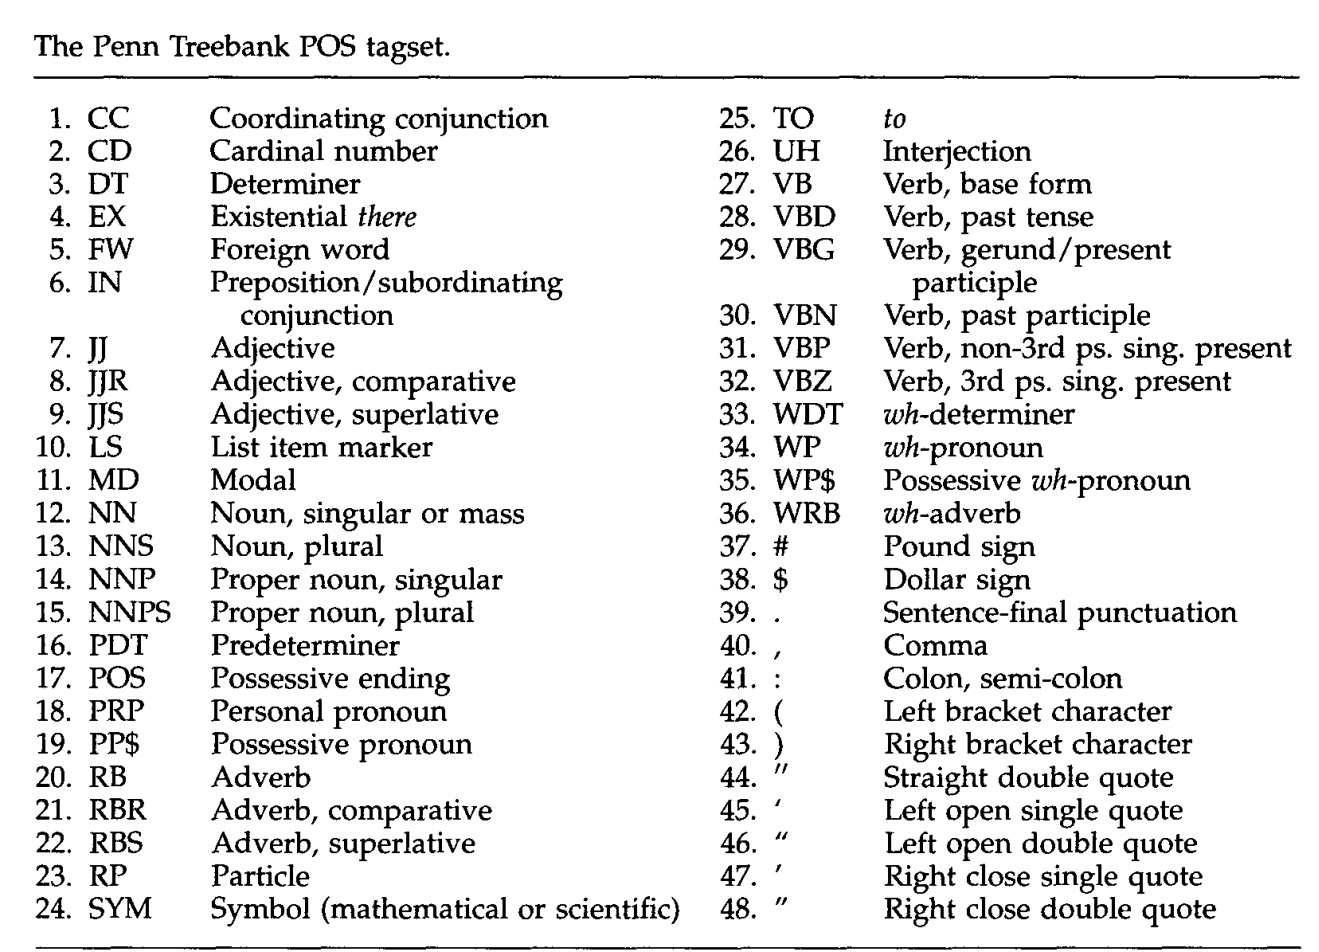
\includegraphics[scale=0.3]{graficos/penn-tagset}
  \caption{Tagset Penn Treebank}
  \label{fig:tagset-penn}
\end{figure}

%\newline

Por su parte, el pos-tagger español de Freeling, por su naturaleza multilingüe, utiliza el tagset propuesto por el grupo EAGLES (\textit{Expert Advisory Group on Language Engineering Standards})\footnote{\url{http://www.ilc.cnr.it/EAGLES96/home.html}}, una organización europea que fomenta la investigación multilingüe, mientras que por una cuestión de compatibilidad, se preservan los tags de Penn Treebank para el inglés. Los tags de EAGLES tienen en consideración diferentes matices para contemplar las variaciones de diferentes idiomas. Sobre un conjunto inicial de 12 categorías -las 9 recién enunciadas más \sq{Signos de puntuación}, \sq{Numerales} y \sq{Fechas y horas} define etiquetas mucho más especificas. En concreto, un tag consta de entre 6 y 7  posiciones, cada una de las cuales expresa una caracteristica de la palabra dependiendo del valor especificado en la posición anterior. Para algunas clases alguno de estos valores no tienen sentido, mientras que para algunas palabras algunos valores no están o no pueden definirse (en el caso de subespecificación de un atributo, esta se nota como un \sq{0}). 
A continuación presentamos la especificación para el conjunto de tags relacionados con sustantivos y un ejemplo de su aplicación.

\begin{center}
\begin{tabular}{| l | l | l | l |}
 \hline
 \multicolumn{4}{|c|}{Nombres} \\ \hline
Pos. & Atributo & Valor & Código \\ \hline
1 & Categoría &  Nombre & N \\ \hline
\multirow{2}{*}{2} & \multirow{2}{*}{Tipo} & Común  & C \\ \cline{3-4}
  & &      Propio & P \\ \hline
\multirow{3}{*}{3} & \multirow{3}{*}{Género} & Masculino & M \\ \cline{3-4}
 & & Femenino &  F \\ \cline{3-4}
 & & Común    & C  \\ \hline
\multirow{3}{*}{4} & \multirow{3}{*}{Número} & Singular & S \\ \cline{3-4}
 & & Plural &  P \\ \cline{3-4}
 & & Invariable & N  \\ \hline
 \multirow{4}{*}{5-6} & \multirow{4}{*}{Clasificación Semántica} & Persona & SP \\ \cline{3-4}
 & & Lugar &  G0 \\ \cline{3-4}
 & & Organización &  O0 \\ \cline{3-4}
 & & Otros & V0  \\ \hline
\multirow{2}{*}{7} & \multirow{2}{*}{Grado} & Aumentativo  & A \\ \cline{3-4}
  & & Disminutivo & D \\ \hline
\end{tabular}
\end{center}


\begin{center}
\begin{tabular}{| l | l | l |}
 \hline
Forma & Lema & Etiqueta \\ \hline 
chico & chico & NCMS000 \\ \hline
chicas & chico & NCFP000 \\ \hline
gatito & gato & NCMS00D \\ \hline
oyente & oyente & NCCS000 \\ \hline
oyentes & oyente & NCCP000 \\ \hline
cortapapeles & cortapapeles &NCMN000 \\ \hline
tesis & tesis & NCFN000 \\ \hline
Barcelona & barcelona & NP000G0 \\ \hline
COI & coi & NP000O0 \\ \hline
Pedro & pedro & NP000P0 \\ \hline
\end{tabular}
\end{center}


Existen varios enfoques algoritmicos al problema del POS tagging: desde los más primitivos basados en reglas escritas a mano pasando a los basados en HMMs (Hidden Markov Models), Maximum Entropy o Transformation Based Learning. Un detalle de estos métodos excede la introducción al problema que supone esta sección de la tesis. El POS tagger de Freeling está basado en el approach de HMMs y el de Stanford en el de Maximum Entropy, ambos modelos de machine learning. En \allref{subsec:freeling-pos} y \allref{sec:stanford-pos} se encuentran algunos comentarios más técnico de los algoritmos de POS tagging que utilizamos en este trabajo y vinculos a bibliografía pertinente y en la sección siguente \allref{subsec:nerc} veremos una descripción más detallada de enfoques algorítmicos al problema que ilustrarán, al menos de modo general, la estructura de la algoritmía basada en machine learning aplicada a procesamiento de lenguajes. 
A continuación listamos ejemplos concretos de análisis de la oración de ejemplo del comienzo de esta sección (\dq{El hombre bajó la escalera.}) para mostrar un funcionamiento real de los algoritmos utilizados en esta tesis. 


\begin{center}
\begin{tabular}{| l | l | l |}
\hline
\multicolumn{3}{|c|}{Freeling (ES)} \\ \hline
Forma &  Etiqueta & Descripción \\ \hline 
El & DA0MS0 & Determinante, Artículo, Másculino, Singular\\ \hline 
hombre & NCMS000 & Nombre, Común, Másculino, Singular  \\ \hline 
bajó & VMIS3S0 & Verbo, Principal, Indicativo, Pasado, Tercera Persona, Singular\\ \hline 
la & DA0FS0 & Determinante, Artículo, Femenino, Singular\\ \hline 
escalera& NCFS000 & Nombre, Común, Femenino, Singular \\ \hline 
.& Fp& Punto final\\ \hline \hline
\multicolumn{3}{|c|}{Freeling (EN)} \\ \hline
Forma & Etiqueta & Descripción \\ \hline 
The &DT & Determiner \\ \hline 
man &NN & Noun, singular or mass \\ \hline 
came  &VBD& Verb, past tense\\ \hline 
down  &RP& Particle \\ \hline 
the &DT& Determiner \\ \hline 
stairs & NNS& Noun, plural \\ \hline 
.& Fp& Sentence final punctuation \\ \hline \hline
\multicolumn{3}{|c|}{Stanford (EN)} \\ \hline
Forma & Etiqueta & Descripción \\ \hline 
The &DT & Determiner \\ \hline 
 man & NN & Noun, singular or mass \\ \hline 
  came &VBD  & Verb, past tense \\ \hline 
 down & RP  &  Particle\\ \hline 
 the & DT  &  Determiner \\ \hline 
 stairs. &NN   & Noun, plural \\ \hline 
 \end{tabular}
\end{center}

En el scope de este proyecto, utilizamos pos-tagging para filtrar clases de palabras inútiles y para seleccionar tres tipos: las qwords, los verbos y los sustantivos (Las qwords son los pronombres interrogativos: qué, quién, cómo, etc. y en inglés, who, when, where...). \newline


\subsection{Reconocimiento de Entidades Nombradas (NER)}
\label{subsec:nerc}
\faltapoco

El reconocimiento de entidades nombradas (NER, de Named Entity
Recognition) es una subtarea de Information Extraction. Information
Extraction es, brevemente, todo el dominio de problemas vinculado con
la extracción de información estructurada a partir de datos no
estructurados o semi estructurados. NER es, dentro de este dominio, el
proceso de reconocer unidades de información (las entidades
nombradas) tales como nombres de personas, organizaciones, lugares,
expresiones numéricas como tiempo, fechas, dinero, porcentajes, etc.
A veces se habla de NERC (Named Entity Recognition and Classification)
para poner énfasis en la asignación de un tipo (por ejemplo: nombre
de empresa) a la entidad nombrada reconocida.

Los primeros sistemas de NER eran algoritmos basados en reglas
hardcodeadas, mientras que los más modernos incorporan técnicas de
machine learning y son, en general, algoritmos basados en features.

El primer sistema data de 1991 y constaba de reglas escritas a mano y
heurísticas simples. Recién en 1996, con el estímulo de la MUC-6
(una conferencia reconocida en el área que dedicó una edición a
NER), el área comenzó a acelerar su crecimiento.

Muchos trabajos sobre NER están basados sólo en inglés, pero también existen trabajos para otros idiomas y, más en general, que buscan la independencia del idioma (o también ser multi-idioma). En la CONLL-2003 (otra conferencia reconocida del área) se trabaja fuertemente el problema NER para el alemán, mientras que en la CONLL-2003 se estudia el español y el holandés y, en general, el estado de arte tiene avances, más o menos prometedores, para una gran variedad de idiomas.

El problema del reconocimiento de entidades nombradas está acotado a lo que el filósofo del lenguaje Saúl Kripke llamó “designador rígido”, dejando afuera las descripciones definidas. Por ejemplo, podemos referirnos a Saúl Kripke como “Saúl Kripke” o como “el filósofo de lenguaje que acuñó el concepto de designador rígido”. El primer ejemplo es un designador rígido y un NER debería detectarlo, mientras que el segundo es una descripción y por lo tanto queda afuera de esta subtarea. Notar que ambos denotan unívocamente a un individuo. Para identificar a la compañía automotriz creada por Henry Ford, dos designadores rígidos son “Ford” y “Ford Company”, etc. Más en general, los designadores rígidos incluyen nombres propios tanto como clases naturales (por ejemplo, especies de biología y nombres de sustancias, etc). Además, se incorpora al problema la detección de expresiones temporales (“26 de Agosto de 2013”) y ciertas expresiones numéricas como dinero (“U\$D 250”) y otros tipos de unidades (“20\%”, “10,25”, etc). En un principio se buscaba detectar nombres propios en general, pero luego se incorporó la clasificación como un paso de esta subtarea. Las clases más utilizadas, por una cuestión completamente pragmática, son: persona, organización y lugar (location). Estas tres clases se conocen con el nombre de ENAMEX. A su vez, existen trabajos que subclasifican estas tres clases, dando como output, para un lugar (location), un subtipo como  “ciudad”, “estado” o  “país” y para personas alguna definición más específica (“político”, “farandulero”, “deportista”, etc). Algunos trabajos incluyen otras clases como “varios”, para aquellos que no caen con un grado alto de confiabilidad en ninguna categoría, y categorías específicas para los valores numéricos (date, time, money, percent, etc). Las categorías estándar pueden, sin embargo, adaptarse a las clases de entidades nombradas de un dominio de problemas puntual, pero por lo general este enfoque requiere del entrenamiento de módulos de machine learning, lo cual suele requerir una serie de inputs de los que no siempre se dispone (principalmente, un corpus de datos suficientemente grande para entrenar el sistema y la disponibilidad temporal para configurarlo).


Además de los ya mencionados sistemas de reconocimiento de entidades nombradas basados en reglas escritas a mano del comienzo de las investigaciones en el área, existen los basados en machine learning, en los cuales vamos a detenernos brevemente en esta sección. Los algoritmos basadon en machine learning son entrenados sobre un corpus de datos con ejemplos positivos y negativos de entidades nombradas, a partir de los cuales infieren sus propias reglas de reconocimiento basadas en features. Hay tres tipos de enfoques al problema basados en machine learning: aprendizaje supervisado , aprendizaje semi supervisado y aprendizaje no supervisado.
El aprendizaje supervisado es la técnica actualmente más utilizada para resolver el problema de reconocimiento de entidades. Estos métodos incluyen Hidden Markov Models (HMM), Decision Trees, Maximum Entropy Models (ME), Support Vector Machines (SVM)  y Conditional Random Fields (CRF). Estos métodos son variantes de un modelo único de aprendizaje supervisado que consiste en leer un gran corpus de datos anotados, crear features de identificación y clasificación de entidades a partir de estos datos (generar un \textit{modelo entrenado}) y finalmente identificar y clasificar un input nuevo en base a este modelo. 

En cuanto al aprendizaje semi supervisado, la principal técnica aplicada a NER es conocida como “bootstraping” e involucra un grado de supervisión bajo, como por ejemplo, configurar un conjunto inicial de semillas (seeds) para el algoritmo de aprendizaje. Un ejemplo típico de este tipo de enfoque puede verse en el algortimo {\color{red} KnowItAll?? explicado en la sección Relation Extraction}. Más genéricamente, un algoritmo de aprendizaje semi automático podría buscar a partir de los ejemplos iniciales (dados manualmente) otras entidades que cumplan el mismo rol léxico en contextos similares, para luego iterar sobre el conjunto ampliado.
Otro enfoque consiste en aplicar una serie de reglas simples basadas en patrones (por ejemplo: “New York” es una entidad de tipo location; si empieza con “Sr.” es una entidad de tipo person”) y luego identificar contextos de uso común sobre un corpus para generar reglas basadas en contextos. Un contexto puede incluir desde el rol semántico de las palabras en cuestión hasta ciertos patrones (como por ejemplo “empezar con ‘Sr.’”).

Finalmente, existen algortimos de reconocimiento de entidades basados en aprendizaje no supervisado. El enfoque típico es el clustering, por ejemplo: agrupar entidades nombradas de diferentes clusters basados en similaridad de contexto.  La forma general consiste en aplicar diferentes recursos léxicos (por ejemplo, Wordnet) sobre patrones léxicos y estadísticas tomadas de un gran corpus no anotado. 

En nuestro trabajo utilizamos los NER taggers de Stanford\cite{NER2} y de Freeling, el primero implementando un algoritmo CRF, es decir, de aprendizaje supervisado (ver \allref{sec:stanford-both}) mientras que el segundo es un algoritmo trivial basado en Autómatas Finitos (ver \allref{subsec:freeling-mods}). Para descripciones y referencias de diferentes implementaciones de algoritmos de NERC ver \cite{NER1}.


\subsection{Clasificación de Preguntas (QC)}
\label{subsec:qc}
\faltapoco
Question Classification es la tarea de categorizar preguntas en diferentes 
clases semánticas que impongan restricciones significativas a las respuestas potenciales 
para utilizarlas en fases posteriores del proceso de QA.
La clasificación de preguntas es una subclase del problema de la clasificación. 
Un clasificador es una herramienta que asigna a un elemento una de
\textit{k} clases. La clasificación es un área bastante fecunda de nlp y, más en general, de machine learning. 
Los clasificadores de preguntas son herramientas que clasifican preguntas según su tipo de respuesta esperada. Por ejemplo:
\dq{?`Quién descubrió América?} espera, más allá del nombre concreto, \textit{un nombre de persona}; {\textquotedblleft}?`Cuándo se descubrió
América?{\textquotedblright} espera \textit{una fecha} (o, más en
general, \textit{un tiempo}), {\textquotedblleft}?`Dónde se
descubrió América?{\textquotedblright} espera, como respuesta,
\textit{un lugar}, etc. Este es un eje de clasificación conocido como
tipo de respuesta esperado, aunque existen otros. Notar que este último ejemplo, en concreto confuso (¿tiene sentido la pregunta?), no lo es a nivel estructural.

El rol del módulo de QC en un sistema de QA es doble: Por un lado, impoen restricciones a la respuesta final, permitiendo filtrar y verificar respuestas candidatas.
Por otra lado, provee información para estructurar el flujo de código de los procesos subsiguientes, permitiendo implementar estrategias puntuales para cada tipo de respuesta esperada. Por ejemplo, para la pregunta \dq{?`Quién fue el primer presidente constitucional de Argentina?} resulta de gran utilidad, a la hora de evaluar pasajes, saber que la respuesta esperada debe ser una \textit{persona}: de este modo se puede evitar el procesamiento lingüístico de un gran dominio de pasajes no relevantes. Estas mismas razones justifican la deseabilidad de la especificidad: saber que la respuesta final debe ser un \textit{presidente} o un \textit{político} es más informativo y útil para el resto del proceso que solo saber que es una \textit{persona}.

Debido a la complejidad de análisis lingüístico intrinseca en la clasificación específica, los sistemas de QC más básicos adoptan un esquema de clases acotado y basado en reglas simples. Típicamente, las clases son: \textit{Persona}, \textit{Lugar}, \textit{Organización}, \textit{Fecha}, \textit{Cantidad}, \textit{Duración}, \textit{Medida}, mientras las reglas de clasificación son parecidas a las siguientes:
\begin{itemize}
\item Si la pregunta empieza con \textit{Quién} o \textit{Quiénes}, entonces el tipo es \textit{Persona}
\item Si la pregunta empieza con \textit{Dónde}, entonces el tipo es \textit{Lugar}
\item Si la pregunta empieza con \textit{Cuándo}, entonces el tipo es \textit{Fecha}
\item Si la pregunta empieza con \textit{Qué}, entonces determinar el tipo de acuerdo al sustantivo principal de la pregunta (utilizando pos-tagging)
\item ...
\end{itemize}

Como nota al pie, este esquema de clasificación semántico es uno entre otros. Por ejemplo, \cite{QC-other} propuso un esquema \textit{conceptual} de 13 clases en las que incluye, por ejemplo: antecedentes y consecuencias causales, habilitación, verificación, disyunción, etc.

Estas reglas básicas -triviales, si se quiere- cubren gran parte de las preguntas con una eficacia alta. En \allref{sec:stanford-qc} veremos un enfoque más complejo que permite una clasificación más granular, basado en machine learning. El uso de algoritmos de machine learning tiene una serie de ventajes interesantes a la hora de definir un sistema de clases complejo. Como mencionamos al hablar de los otros taggers, la definición de reglas manuales es una tarea tediosa y con poca capacidad de adaptarse o modificarse, mientras que la definición de un set de features adecuado para el aprendizaje programático, en cambio, permite la fácil incorporación de nuevas clases y/o la incorporación de nuevas mejoras descubiertas. Por otro lado, un esquema de clases semánticamente rico -más granular que el modelo básico recién enunciado- requiere la consideración de una gran cantidad de dimensiones lingüísticas, tanto sintácticas como semánticas, lo que hace que la definición manual de reglas una tarea potencialmente imposible en terminos de costo de tiempo humano. 

Finalmente, cabe mencionar que no existen clasificadores de preguntas para el español y que a la hora de abordar este problema en nuestra implementación debimos apelar a mecanismos ad-hoc. En particular, para el modelo estructurado implementamos un sistema de reglas simples como el recién enunciado y para el modelo no estructurado utilizamos el resultado de la clasificación de la misma pregunta pero formulada en inglés (pues las preguntas están disponibles en ambos idiomas).
Actualmente, un tesista del grupo GALLI está trabajando en la construcción de un corpus para alimentar un clasificador de preguntas basado en machine learning para el español, pero lamentablemente por cuestiones de tiempos no pudimos hacer uso del mismo en esta tesis.


\subsection{Otras tareas}
\horriblearg{Volar?}
\begin{itemize}
\item Detecci\'on de idioma
\item Tokenizer
\item Sentence splitting,
\item Análisis morfol\'ogico
\item NER y NEC (Detecci\'on y Clasificaci\'on de Entidades Nombradas)
\item Reconocimiento de fechas, números, magnitudes físicas, monedas
\item Codificaci\'on fonética
\item POS tagging, 
\item Shallow parsing
\item Dependency parsing
\item Wordnet-based sense annotation
\item Word Sense Disambiguation
\item Coreference resolution
\end{itemize}

Esta sección es un placeholder para las siguientes posibles tecnologías que podría describirse como última sección en \allref{chap:teorico}
\begin{itemize}
  \item Coreference Resolution \\
  Ejemplos de resolución de Freeling.
  \item Word sense disambiguation \\
  Hablar algo de wordnet?
  \item Relation Extraction \\
  La detección y extracción de relaciones es una tarea de procesamiento
de lenguaje natural que consiste en extraer entidades y relaciones semánticas
entre entidades a partir de un texto no estructurado. 

[[Escribir sobre distintos algoritmos conocidos basado en el paper RE1]]
  \item Machine Translation \\
    Hablar de los problemas con Google y otros y de las memorias de traducción. 
  \item Detección de idiomas \\
  La detección o identificación de idioma es la tarea de reconocer el
idioma de un cierto contenido. Esta tarea puede pensarse como una
tarea de clasificación donde las clases son los distintos
idiomas que el detector puede reconocer. 
  \item Shallow parsing (also chunking, "light parsing") \\
  is an analysis of a sentence which identifies the constituents (noun groups, verbs, verb groups, etc.), but does not specify their internal structure, nor their role in the main sentence.
It is a technique widely used in natural language processing. It is similar to the concept of lexical analysis for computer languages.
[[Expandir con detalles técnicos de wikipedia]]
\end{itemize}

ReVerb is a program that automatically identifies and extracts binary relationships from English sentences. ReVerb is designed for Web-scale information extraction, where the target relations cannot be specified in advance and speed is important.

ReVerb takes raw text as input, and outputs (argument1, relation phrase, argument2) triples. For example, given the sentence "Bananas are an excellent source of potassium," ReVerb will extract the triple (bananas, be source of, potassium).
